\documentclass[12pt]{article}
\usepackage{hyperref}
\usepackage{graphicx}
\usepackage[font=small,labelfont=bf]{caption}
\title{Progetto di fine corso}
\date{17/05/2016}
\author{Alessio Luca,Carlo Sindico}

\begin{document}
	\pagenumbering{arabic}
	
	\begin{titlepage}
		\newcommand{\HRule}{\rule{\linewidth}{0.5mm}}%linea orizzontale
		\center
		
		\textsc{\LARGE Universit\`a degli Studi di Padova}\\[1.5cm] 
		\textsc{\Large Laurea in Informatica}\\[0.5cm]
		\textsc{\large Corso di Tecnologie Web}\\[0.5cm]
		\textsc{\large Progetto di fine corso}\\[0.5cm]
		
		%----------------------------------------------------------------------------------------
		%	TITLE SECTION
		%----------------------------------------------------------------------------------------
		
		\HRule \\[0.4cm]
		{ \huge  2FORCHETTE}\\[0.3cm] 
		\HRule \\[0.4cm]
		
		
		%----------------------------------------------------------------------------------------
		%	AUTHOR SECTION
		%----------------------------------------------------------------------------------------
		
		\begin{minipage}{0.3\textwidth}
			\begin{flushleft} \large
				\emph{Studente:}\\
				Luca \textsc{Alessio} % Your name
			\end{flushleft}
		\end{minipage}
		~
		\begin{minipage}{0.3\textwidth}
			\begin{flushright} \large
				\emph{Matricola:} \\
				\textsc{1070690} % Supervisor's Name
			\end{flushright}
		\end{minipage}\\[2cm]
		
			\begin{minipage}{0.3\textwidth}
				\begin{flushleft} \large
					\emph{Studente:}\\
					Carlo \textsc{Sindico} % Your name
				\end{flushleft}
			\end{minipage}
			~
			\begin{minipage}{0.3\textwidth}
				\begin{flushright} \large
					\emph{Matricola:} \\
					\textsc{1069322} % Supervisor's Name
				\end{flushright}
			\end{minipage}\\[2cm]
			
		%----------------------------------------------------------------------------------------
		%	INFORMATION WEBSITE
		%----------------------------------------------------------------------------------------
		
		\textsc{\Large Informazioni sul sito:}\\[0.3cm]	
		\textsc{http://tecnologie-web.studenti.math.unipd.it/tecweb/~csindico/}\\[1cm]
		
		%----------------------------------------------------------------------------------------
		%	DATI LOGIN
		%----------------------------------------------------------------------------------------
		
			\textsc{\Large Dati login:}\\[0.3cm]
			\textsc{ Username:Admin}\\[0.1mm]
			\textsc{ Password:Admin}\\[0.1mm]
			
		\vfill
	\end{titlepage}
	
	\newpage
	\renewcommand{\contentsname}{Indice}
	\tableofcontents
	
	
	\newpage
	\pagenumbering{arabic}
	
	\section{Abstract}
	\begin{itemize}
		\item Il progetto si propone di offrire  alla maggior parte degli utenti  un sito che ha come contenuto un insieme di ricette. 
			
		Il sito ha un scopo principalmente informativo, infatti riporta tutte le informazioni reltaive a ciascuna ricetta. Le ricette sono classificate in Primi piatti, Secondi piatti, Antipasti e Dessert. L'utente ha la possibilit\'a di proporre una nuova ricetta compilando un apposito form, e un lato amministratore ha il pieno controllo nell'accettare o rifiutare le ricette proposte. Si \'e trovato utile inserire una sezione commenti, che permette all'utente di chiedere ulteriori informazioni e inviare feedback scrivendo direttamente nel sito, e l'amministratore ha la possibilit\'a di rimuovere i commenti inopportuni.
		
		Il sito \'e stato creato con lo scopo di essere visualizzato in internet, quindi si \'e data importanza alla presentazione e alla sua usabilit\'a, rispettando lo standard W3C. Infatti si \'e data particolare attenzione nella separazione tra struttura presentazione e comportamento con le regole di accessibilit\'a richieste.
	\end{itemize}
		\section{Utenti destinatari}
		\begin{itemize}
			\item Il sito 
		\end{itemize}
		\section{Accessibilit\`a}
		\subsection{Separazione tra struttura,presentazione e comportamento}
		\begin{itemize}
			\item Per una maggiore accessibilit\'a al sito da parte di utenti disabili e per favorire gli algoritmi dei motori di ricerca si \'e deciso di separarare la struttura dalla presentazione e dal comportamento.
			Infatti il contenuto del sito \'e rapprentato dai file HTML e CGI, i quali richiamano i fogli di stile CSS e si utilizzano (anche in questo caso attraverso percorsi esterni), esternamente controlli in JavaScript in particolare per la compilazione dei form. Tuttavi il contenuto rimane accessibile anche se JavaScript \'e disabilitato.(da verificare!!)
			
			Tutto il codice \'e stato scritto secondo le raccomandazioni W3C,con opportuna validazione di esso.
		\end{itemize}
			\subsection{Colori}
			\begin{itemize}
				\item Si \'e scelto uno schema di colori non particolarmente vivace (arancione opaco,bianco sporco,nero);Non sono colori di base, ma comunque la lettura dei testi risulta accessibile.Bisogna ricordare che si tratta di un sito di cucina e quindi l'utente si aspetta dei colori vivaci adatti al tipo di sito.(da rivedere!!).Inoltre i link sono sempre sottolineati, e diventano del colore standard quando vengono cliccati.
				Di seguito sono riportate le visualizzazioni del sito attraverso alcuni disturbi visivi:
				
			
			\begin{figure}[ht!]
				\centering
				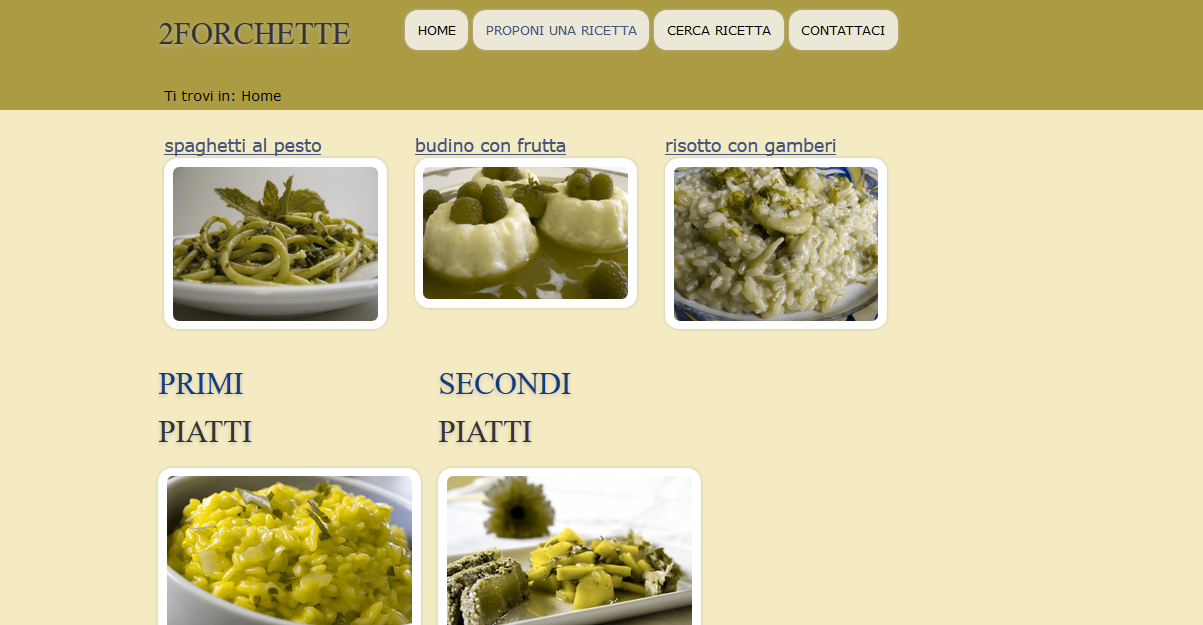
\includegraphics[width=100mm]{test1}
				\caption{vedi file test1.png}
			\end{figure}

				\begin{figure}[ht!]
					\centering
					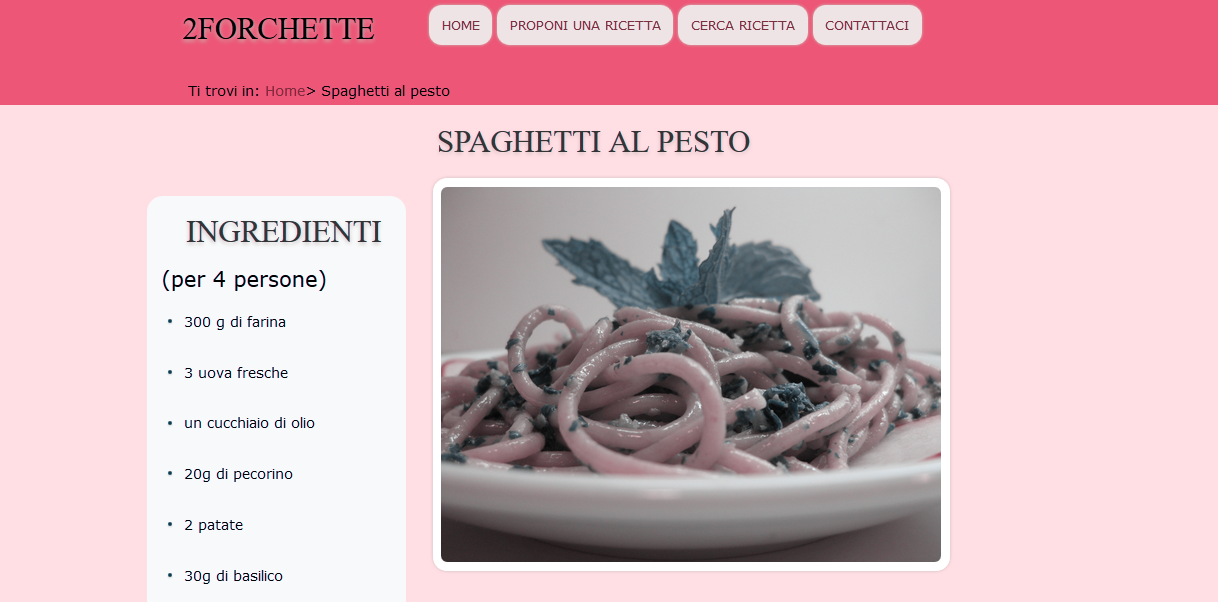
\includegraphics[width=100mm]{test2}					\caption{vedi file test2.png}
				\end{figure}
			\end{itemize}
			\subsection{Tag meta}
			\begin{itemize}
				\item Sono stati inseriti per ogni pagina i tag meta: title, description,keywords,language,author,content-type.
				il tag title descrive la pagina corrente dal particolare al generale.Il tag description da una descrizione del contenuto del sito, il tag language indica che il sito \'e stato interamente scritto in italiano. Compaiono per\'o alcune parole inglesi che sono state segnalate agli screenreader attraverso il tag "span xml:lang=en" segnalando la lingua con cui leggere correttamente i vocaboli. 
			\end{itemize}
			\subsection{Screen reader}
			\begin{itemize}
				\item Ogni foto ha il suo attributo alt che descrive ci\'o che l'immagine ritrae.
				Si è evitato di utilizzare immagini per visualizzare il testo, quindi il contenuto informativo rimane accessibile anche quando fallisce il caricamento delle immagini o del CSS.
			\end{itemize}
			\section{Usabilit\`a}
			\begin{itemize}
				\item Per l'usabilit\`a del sito si è fatta attenzione ad inserire le 6W del giornalismo:
				
				What?: Un utente appena entra nella home capisce subito che si tratta di un sito di ricette, dalla barra dei men\'u (Proponi ricetta, Cerca ricetta), e dal contenuto in primo piano che mette in evidenza alcune ricette proposte.
				
				Who?: A chi \'e rivolto il sito? Il sito grazie alle immagini si capisce che \'e dedicato a mamme e pap\`a
				che vogliono preparare una gustosa ricetta per i propri figli.
				
				Where?: Nonnostante il sito non abbia una propria locazione, gi\'a  nel footer di ogni pagina sono presenti informazioni riguardo gli amministratori e il sito.Per maggiore visibilit\`a, \'e stata inserita una pagina CONTATTACI dove oltre ala sezione commenti, sono specificati gli indirizzi email e numero di telefono degli amministratori. 
				
				When?: ..........
				
				Why?: Perch\'e un utente dovrebbe rimanere nel sito o dovrebbe ritornarci? Il sito \'e principalmente espositivo,(gli utenti possono liberamente visualizzare le ricette), si \'e cercato di renderlo pi\'u interessante, aggiungendo una sezione proponi ricetta (l'utente ha la possibilit\'a di inserire la propria ricetta), e anche una sezione commenti.
				
				How?: La barra di navigazione mostra tutte le sezioni principali del sito alle quali un utente pu\'o accedere.
				
				Nella barra men\'u \'e sempre evidenziata la voce della pagina in cui ci troviamo (DA SISTEMARE),e si vede attraverso una diversa colorazione dei link in quali altre pagine si \'e stati. il testo \'e sottolineato, per evidenziare il fatto che sono link.
				
				Breadcrumbs: Affinch\'e l'utente non si perda mai all'interno del sito, \'e stato riportato sotto la barra di navigazione, il percorso che si \'e effettuato dall'home page.
				
			\end{itemize}
			\section{Gerarchia dei file}
			\begin{itemize}
				\item I file del nostro sito sono organizzati su 3 cartelle:
				\item cgi-bin: cartella nella quale sono presenti i file .cgi con la libreria di supporto.
				\item data: in questa cartella sono contenuti i file xml ed i relativi XMLSchema.
				\item public-html: cartella nella quale sono presenti i file .html e le sotto-cartelle:
				➔ css: cartella contenente i file .css;
				➔ img: cartella contenente tutte le foto del sito;
				➔ js: cartella contenente i vari script realizzati in JavaScript.
			\end{itemize}
			\section{Struttura}
			\begin{itemize}
				\item Nella cartella public-html si trovano i file delle pagine statiche html.
				Le pagine web del progetto sono state realizzate interamente secondo lo standard XHTML 1.0 Strict. Di seguito sono elenate le pagine statiche del sito:
				\begin{itemize} \item index.html: \'e la pagina principale del sito, la Homepage.
					\end{itemize}
				
				\'E importante fare notare che la maggior parte delle pagine sono dinamiche scritte in Perl.(scelta che \'e stata fatta all'inizio).
				Nella cartella cgi-bin invece abbiamo le pagine dinamiche .cgi:
				\begin{itemize} \item proponiricetta.cgi: \'e la pagina nella quale l'utente ha la possibilit\'a di inviare la propria ricetta.
				\end{itemize}
				\begin{itemize} \item cercaricetta.cgi: \'e la pagina nella quale l'utente ha la possibilit\'a di cercare la ricetta che gli interessa.
				\end{itemize}
				\begin{itemize} \item contattaci.cgi: Sezione dedicata all'invio di commenti da parte dell'utente. Sono presenti anche informazioni su come contattare gli amministratori del sito.
				\end{itemize}
				\begin{itemize} \item Primo.cgi: \'e la pagina nella quale l'utente pu\'o sfogliare un elenco di ricette di primi piatti.
				\end{itemize}
				\begin{itemize} \item Secondi.cgi: \'e la pagina nella quale l'utente pu\'o sfogliare un elenco di ricette di secondi piatti.
				\end{itemize}
				\begin{itemize} \item Antipasti.cgi: \'e la pagina nella quale l'utente pu\'o sfogliare un elenco di ricette di Antipasti salati.
				\end{itemize}
				\begin{itemize} \item Dessert.cgi: \'e la pagina nella quale l'utente pu\'o sfogliare un elenco di ricette di Dessert prevalentemente ricette di dolci.
				\end{itemize}
				Fanno parte della cartella cgi-bin altri file che gestiscono la parte dinamica del sito, ad esempio l'invio della ricetta e il salvataggio dei dati nel file XML.
				
			\end{itemize}
			
			\section{Presentazione}
			\begin{itemize}
				\item Nella realizzazione dell'interfaccia grafica del sito è stato usato lo standard CSS3, allo stesso tempo si \'e fatta molta attenzione alla compatibilit\'a con browser pi\'u datati, e si \'e cercato di utilizzare un numero ristretto delle nuove funzionalit\'a offerte dallo standard.
				
				Alcune delle funzionalit\'a CSS3 che sono state utilizzate:
				Border-radius e Box shadow: per realizzare i pulsanti delle form , e per le immagini.
				(DA COMPLETARE!!)
				
			\end{itemize}
			\subsection{Divisione dei file}
			\begin{itemize}
				\item Nella cartella public-html/css sono presenti i seguenti fogli di stile:
				style.css: modella lo stile di visualizzazione del sito ia per gli utenti desktop (che hanno uno schermo largo al massimo 890px) che per gli utenti mobile con dispositivi con schermo piccolo (che hanno uno schermo largo massimo 330px) e dispositivi con dimensioni schermo intermedie (min-width=330px e max-width=550px).(DA RIVEDERE!)
				print.css: modella lo stile di stampa delle pagine del sito.(particolare attenzione si \'e data alla stampa delle pagine delle ricette).
				\end{itemize}
			\section{Comportamento}
			\begin{itemize}
				\item Nel programmare il sito si \'e cercato per quanto possibile di fornire all'utente semplicit\'a, cercando di essere il meno invasivi possibile, per dare una migliore usabilit\'a al sito oltre che una presentazione migliore.
				
				Si \'e fatto uso della tecnologia JavaScript e si \'e cercato di non usare framework o altre tecnologie pi\'u invasive.
				
				JavaScript \'e stato utilizzato per eseguire i controlli sui form, oltre ovviamente all'utilizzo di Perl, questa combinazione \'e dettata dall'esigenza di fornire una risposta pi\'u immediata all'utente. Anche senza Javascript comunque non vi \'e la possibilit\'a che siano memorizzati dati con caratteri che compromettono la validazione del sito o che siano vuoti dove il campo invece non debba esserlo.
				Anche se JavaScript non è comunque necessario per il corretto funzionamento del sito, migliora
				l'usabilità generale, in quanto oltre a dare una risposta più immediata, visualizza anche una breve
				descrizione di ciò che si vuole sia inserito nel campo, quindi è presente un avviso che invita ad
				attivarlo implementato tramite tag noscript nei form dove esso è di utilità.
				JavaScript esegue quindi i controlli che sono più di interesse per l'utente, atti soprattutto a verificare
				se un campo è vuoto, e l'output di queste valutazioni è visualizzato in uno spazio apposito vicino al
				campo che ha generato l'errore.
				Si è  deciso di non  ricorrere il meno possibile agli alert di JavaScript, in quanto essi sono finestre
				popup, che sono odiate dagli utenti web e il cui utilizzo estensivo quindi avrebbe compromesso
				fortemente l'usabilità e l'attrattiva del sito.
				
				
				Si è scelto di attivare questi controlli in reazione all'evento onsubmit, in quanto permette un
				fallback semplicissimo in caso JavaScript non sia supportato. Quindi tutte le funzioni ritornano il
				valore false se i controlli non sono superati e true se invece sono stati superati tutti i controlli.
				
				Le funzioni sono contenute nei file:
				\begin{itemize}
					\item proponiricetta.js, che esegue i controlli relativi ai campi, non effettua controlli sull'immagine in quanto la gestione di tale parte \'e affidata al Perl.
				\end{itemize}
				\begin{itemize}
					\item validacommento.js, che esegue controlli relativi ai campi, e scrive del testo di aiuto se sono sbagliati. Controlla che il formato mail sia valido, se inserita. Questo ultimo controllo non viene eseguito dal Perl, in quanto si tratta di un campo facoltativo e quindi un'email non corretta non genere alcun tipo di problema. 
				\end{itemize}
				\begin{itemize}
					\item logincontrol.js, che esegue i controlli sui campi e verifica che non siano vuoti.
				\end{itemize}	
			\end{itemize}
		
		\section{Gestione dei dati}
		\begin{itemize}
			\item Il sito presenta due tipi di contenuto che posso essere modificati.
			Tutti quanti possono scrivere commenti, e proporre ricette. Non \'e necessaria l'autenticazione per fare queste due operazioni, in quanto si \'e ritenuto che dover far registrare un utente solo per avere la possibilit\'a di inserire un commento o proporre una ricetta era una richiesta eccessiva, che impattava l'usabilit\'a e che sarebbe malvista dagli pubblico.D'altronde la ricetta che \'e proposta dall'utente non viene subito resa visibile, ma passa sotto il controllo dell'amministratore prima di essere pubblicata.
			Per i commenti il pubblico deve fornire un nome per identificarsi.
			
			
			Agli utenti autorizzati (l'amministratore del sito) \'e invece concessa la possibilit\'a di rimuovere oppure accettare le ricette proposte, e di rimuovere i commenti inappropriati.
		\end{itemize}
			
			
			
				
		
	
	
\end{document}